\chapter{Introduction}
\label{chap-1-intro}
\begin{ChapAbstract}
In this chapter, we talk about overview of our study, from remote sensing introduction, related work to our contributions. At the end, this thesis's outlines is also provided.

\end{ChapAbstract}


\section{Overview} 

Remote sensing, and satellite images in particular, has become an indispensable part in our daily life. Many different techniques can be used to apply on these kind of data, in order to monitor or measure phenomena found in the lithosphere, biosphere, hydrosphere and atmosphere. With the help of mechanical devices, which are known as remote sensors, the huge and diverse amount of data was collected by many satellite. NASA, who has many public satellites programs, have been proved invaluable to the research community. For example, Landsat program is one of them where its images of the Earth surface since 1984 with high resolution (from 10m to 30m per pixel) have been made publicly  free of charge. Recently ESA (European Space Agency) has endeavored a similar but more ambitious program called Corpernicus in which a series of Sentinel satellites have been launched since 2014.

Remote sensing imagery has many applications in mapping land-use and cover, soils, forestry, city mapping and monitoring, archaeological investigations, geomorphological surveying and so on. For example, foresters use aerial photographs for preparing forest cover maps, locating possible access roads, and measuring quantities of trees harvested. Specialized photography using color infrared film has also been used to detect disease and insect damage in forest trees. 

With more modern device nowadays, it is able to collect image data with better quality, higher resolution, and on multiple bands covering lands, waters, seas, and atmosphere. Our study is projected into those advances and to be expected to gain a better understanding the complex of water cycle under human impact, with help of Machine Learning.


\section{Introduction to Remote Sensing} % 2 pages

As we known, remote sensing imagery is the data that acquired from satellites on the sky. The uses of those data might be making surface map (for examples: Google Maps, Apple Map); creating maps of land surface temperature, reflectance and elevation; monitoring hydrology and land changes, etc. 

The Two of most popular between many kinds of satellites are optical-type and radar-type.

\subsection{Optical satellites}

Satellites with optical sensors provide images of the Earth over relatively large areas and are useful in the production of hydrology and vegetation maps. The sensors function in the optical part of wavelength spectrum, including visible, near infrared and short-wave infrared wavelengths. Satellite sensors commonly used for detailed mapping include Landsat, Sentinel-2, etc., with moderate resolution (resolution is approximately from 10 to 30 meters).

\begin{figure}
\centering
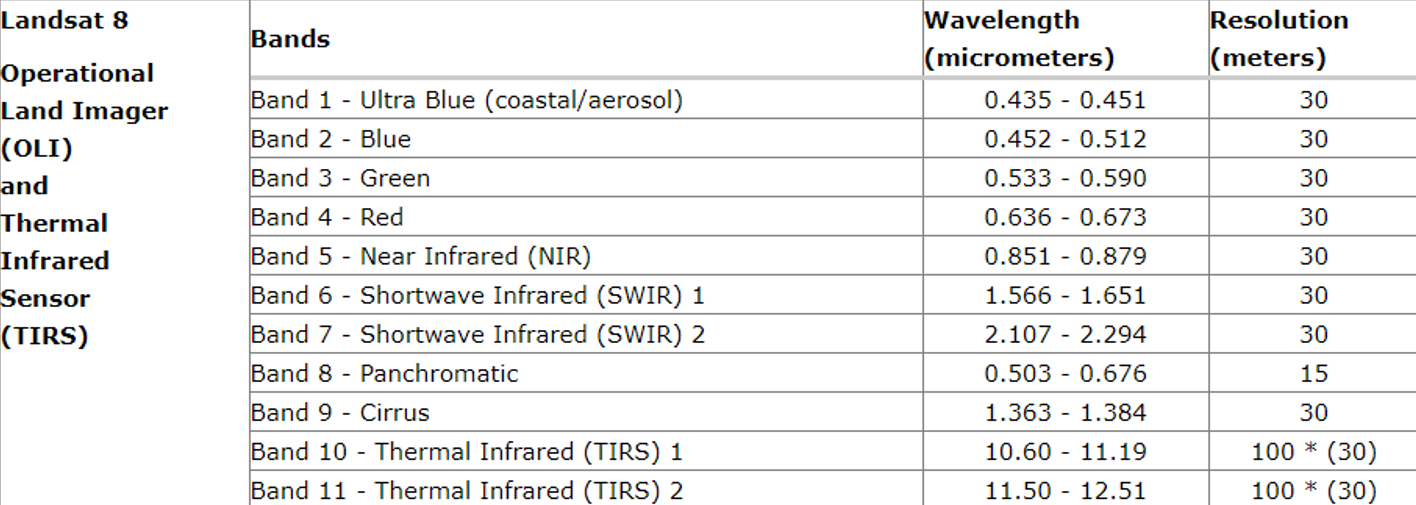
\includegraphics[width=0.7\linewidth]{figures/wavelengthL8.png}
\caption{Landsat 8 data specification. Source: USGS}
\end{figure}

Wavelengths of optical satellites are useful for distinguishing between forest types and other vegetation classes. Optical satellite data can be combined with laser data because the color information in optical satellite data can distinguish different vegetation types while laser data provides additional information about terrain or vegetation characteristics. 

\begin{figure}[h!]
\centering
\subfloat[True Color]{
	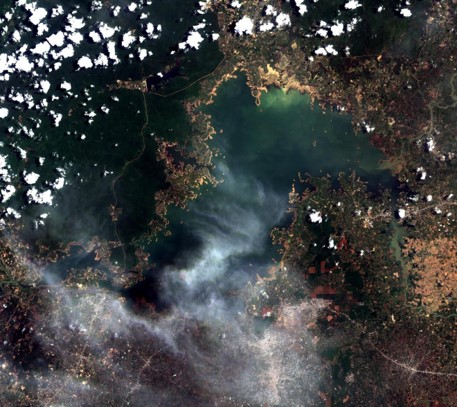
\includegraphics[width=0.24\linewidth]{figures/trueColor.jpg}
} 
\subfloat[Land/Water]{
	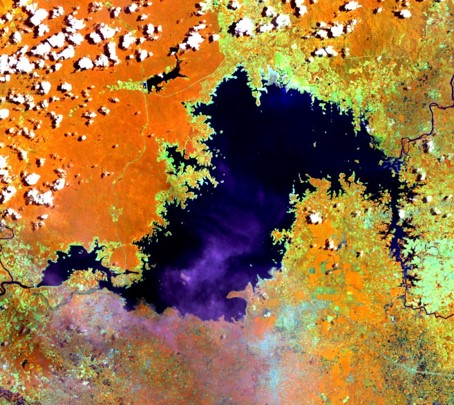
\includegraphics[width=0.24\linewidth]{figures/landwater.jpg}
}
\subfloat[Normalized difference water index]{
	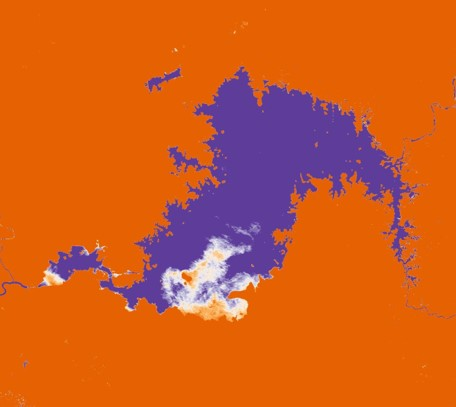
\includegraphics[width=0.24\linewidth]{figures/ndwi.jpg}
} 
\subfloat[Agriculture]{
	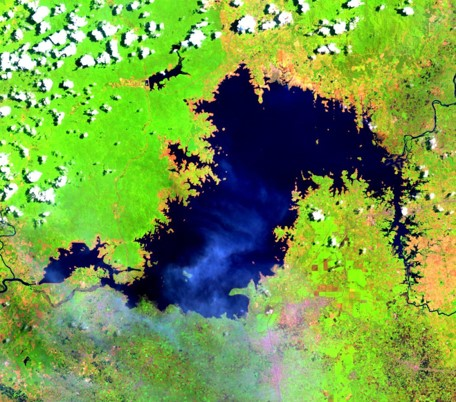
\includegraphics[width=0.24\linewidth]{figures/agriculture.jpg}
}
\centering
\caption{Samples of bands combinations from Landsat 8 data files:
\textbf{(a)} (B4, B3, B2), \textbf{(b)} (B5, B6, B4), \textbf{(c)} (B3 - B5)(B3 + B5), \textbf{(d)} (B6, B5, B2).}
\end{figure}

\subparagraph{Addition: The Landsat 8 Pre-Collection Quality Assessment (QA) band}

QA band is a part of Landsat 8 data files. Each pixel in the QA band contains integer that represent bit-packed combination of surface, atmosphere and sensor conditions that can affect overall usefulness of a given pixel. Depending on its pixel value (mostly depending on QA Bits), we can detect that pixel is a snow/ice, cloud or water (because these are mainly formed by water) or detect the cloud direction due to cirrus confidence. For more information about QA Band, see at: \href{https://landsat.usgs.gov/qualityband}{https://landsat.usgs.gov/qualityband}.

\begin{figure}
	\centering
	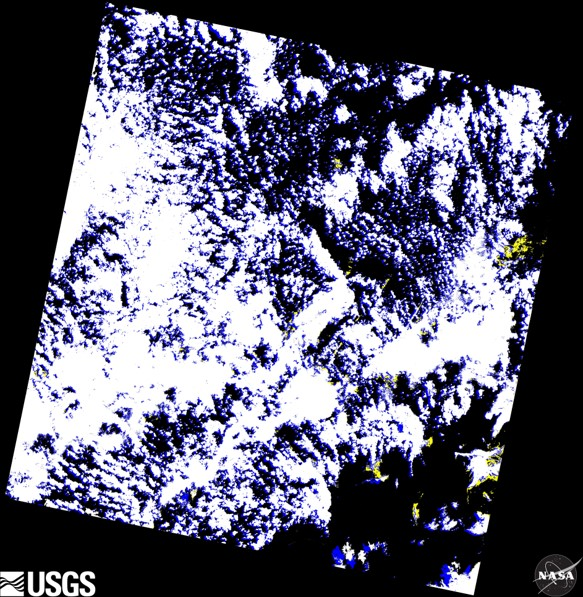
\includegraphics[width=0.32\textwidth]{figures/qaL8.jpg}
	\caption{Landsat 8 QA Band, Tri An Reservoir. Date taken: May 30, 2017}
\end{figure}

\subsection{Radar satellites}

Radar satellites can solve problem of satellites image on cloud days, and this is the biggest advantage of radar data over optical data. They are not affected by cloud because of its instrument specifications. For example, Sentinel-1 satellites use the C-Band Synthetic Aperture Radar (SAR). This colored Sentinel-1 SAR image is produced by showing the two polarisations (VV and VH i.e. vertical polarisation send for the radar signal and vertical or horizontal receive). 

\begin{figure}[h!]
	\centering
	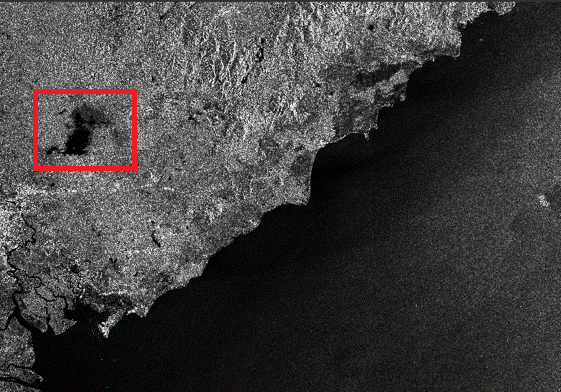
\includegraphics[width=0.6\textwidth]{figures/sarImgVVS1.png}
	\caption{Sentinel-1 (band VV) image, Tri An Reservoir. Date taken: June 11, 2017}
\end{figure}	

With the initial goal of monitoring reservoirs, SAR images seem to be the swiss knife to our problem until it is put in the context of machine learning the hydrological cycle of reservoirs for prediction. A long times-series of satellite images is the prerequisite to detect such patterns and therefore when it comes to SAR images the data source is very scarce. The Sentinel-1 satellites coverage is just from 2014. Other SAR image sources are costly or nontrivial to access. This makes a strong motivation for us to achieve a robust  method that remove clouds from multi-spectral satellite images and make them useful for monitoring purpose. From this point of view, a long term data source such as of Landsat-5, 7, and 8 is very useful to understand the water cycle of reservoir which is often complex by hydrological, economical, and political factors. Furthermore, multi-spectral images are useful in monitoring vegetation, which is closely related to the amount of water being used from reservoirs for irrigation. Ideally multi-spectral data can be combined with SAR data to provide the best temporal coverage and help to distinguish vegetation types while laser data provides additional information about water content in soil. 


\section{Related Work} % 2 pages

% \textbf{Thêm hình vào}

% Water Resources Monitoring problems and application. ~2 paper

Water resources monitoring provides information about the state and trend of monitored objects, which are water bodies a.k.a lakes, rivers or reservoirs on the Earth. It might be:

\begin{itemize}
	\item \textit{a local monitoring}, which can give a solution for specific local problem, on a limited part of water body or area.
	\item \textit{a global monitoring} on larger area, which has state that could be impacted or caused by some human activities.
	\item \textit{comprehensive monitoring}, which performs on a network of multi water body observation, in order to make decision for efficient use, protection and restoration of water resources.
	\item \textit{disaster monitoring}, which could immediately warn about anomaly situation on water body area, loads, etc., primarily by human activities.
\end{itemize}

Nowadays remote sensing techniques, when combines with Computing, they are used in different area of research for monitoring. For examples with internet of Things (IoT), a smart water quality monitoring system for Fuji Islands, located in the vast Pacific Ocean, is proposed in \cite{Prasad2015}. Besides that, water level monitoring and management of dams \cite{Sreekar2018} could help people on automatically closing or opening gate of the dam, depending on current water level in dams is less or higher than optimum value.

\subparagraph{Water body segmentation problems} In order to reach above aims, many different water body segmentation techniques are widely used. Each techniques could be used on some certain types. For example with multi-spectral data like Landsat, an automatic mapping water bodies approach to detect waterline boundaries is proposed in \cite{Verpoorter2012}, or applying Principle Component Analysis, which is a famous image processing technique to find out most important dimensions of data, to find out segmentation and morphology of open water bodies \cite{Jorge2006}. There are also many approaches for radar optical images. With SAR images provided by Sentinel-1, water volumes retained at reservoirs can be monitored after creating an interferometric of area \cite{Amitrano2014}, detect surface water bodies using Valley-Emphasis method \cite{Nguyen2016}.

\subparagraph{Water body recovery problems} Due to limitations of optical satellites like Landsat, MODIS, on the days that surface is covered by thick clouds, the acquired image from those devices usually suffer missing information, caused to not able to use because we can't see anything under cloudy cover. This lead to many problems on segmentation system which uses images from those satellites. In order to solve this problems, many methods have been proposed in order to recover the missing data. This kind of problem is similar to 
in-painting method in image processing field. There are variety of approaches, from using a multi-channel non-local total variation model \cite{Cheng2014}, to applying neural networks to recover\cite{Zhang2018}. Almost these method use one or more undamaged images as reference. 

\subparagraph{Prediction problems} Another problem that Machine Learning, especially Artificial Intelligence has an attractable performance is weather forecasting, a sub-prediction problem. Weather forecasting focuses mainly on the prediction of weather conditions, such as wind direction, wind speed, humidity, rainfall, temperature etc., in the given future time. In Stanford University, a temperature attribute in term of the maximum and minimum value, is being predicted in next seven days, given weather data for the past two days \cite{Holmstrom2016MachineLA}, using Regression Model. A survey of existing research on applying Artificial Neural Networks (ANNs) to weather prediction is also presented \cite{Culclasure2013UsingNN}.

\section{Contributions} % 1 pages

In this thesis, we would like to apply solutions from prediction problems, in order to solve the following things for goal of monitoring reservoirs:

\begin{itemize}
	\item \textit{Water body recovery problems}, As we've known, to predict a missing area in a remote sensing, we need to have at least one image called \textbf{reference}, containing about spectral, spatial or temporal information  (the temporal information only reflects the image in another point of time in the past). Water body is mainly affected by weather and other conditions, such as water flow from other rivers to the lake, elevation and altitude of reservoir, etc. Time-series of data may provide the \textit{periodicity} or at least \textbf{trend} of water body, for example its area is increasing or decreasing, it usually has a large or small area of water body in some months. So that, we will try to apply a periodicity of weather in order to get higher accuracy in \ref{chap-3-recover-water-body}.

	\item \textit{Monitoring water body problems} Another thing that we could analyze from predicted image is about the shape, area, volume and so on. We could compare these aspects with the same time in the past (for an example, the related month in the previous year). This leads to a very famous problem \textbf{Anomaly Detection}. This problems is not only famous in data science, but also in remote sensing\cite{Grosklos2015,Yang2019}. If the techniques used in detection methods are good enough, the monitoring system will help us quickly detect strange scenarios in remote sensing time-series data. This results can be applied in many sectors such as water resource management, irrigation, and disaster prediction and prevention. The latter application is also our long-term goal where a network of interconnected reservoirs and dams  within a river basin are being monitored in order to derive from short to mid-term prediction of water level.
\end{itemize}


\section{Outlines} 

.... 
